\section{Feature Specification}
For this project I initially set out to implement several  different dynamic programming problems into Java programs with helpful output. To begin with I primarily researched into the topic and looked into a variety of problems that I could possibly implement. After making a list of problems I found to be applicable to possibly be covered through this project and producing minimal notation on each of them, I narrowed the list down to ten problems. The initial stages of software design were spent understanding the problems in greater detail and documenting their workings. This then allowed more confidence when it came to actually start properly coding the problems as well as saving time when it came to writing up about each problem for the implementation section of this dissertation.
\smallbreak
While each of the ten programs have their own set of specifications, the basic shared feature that each of them require was to be able to solve the given problem by taking in appropriate input. For each problem this was achieved by having the program's core dynamic programming algorithm work correctly and to then return either true or false, or the length of the answer according to what data was input for which separate program. Additionally the optional feature I set out for each program to have was expanded output, so instead of returning simply true or false, more useful data could be output. As an example, the first program I implemented was the minimum coin change problem. Initially my main focus was on developing the dynamic programming algorithm and in such once I got that working the output was minimal, simply returning the minimum number of coins required to make change for a given amount. However I then expanded the code and ended up producing better output which also returned the values of each of the minimum number of coins required to make change for a given amount.
\smallbreak
Another key feature was for each of the problems to be commented to a satisfying level. My aim was to provide high quality Java comments which would be able to assist in helping somebody understand the specific dynamic programming problem. As I had researched a lot into how these problems are structured and how to go about the problem-solving process, I made sure to write detailed comments for each program and continually update them as I changed the programs around. I also included Javadoc comments for each class and method to keep the code and comments to a professional standard as well as achieving a higher level of user-friendliness.

\begin{figure}[h]
	\centering
	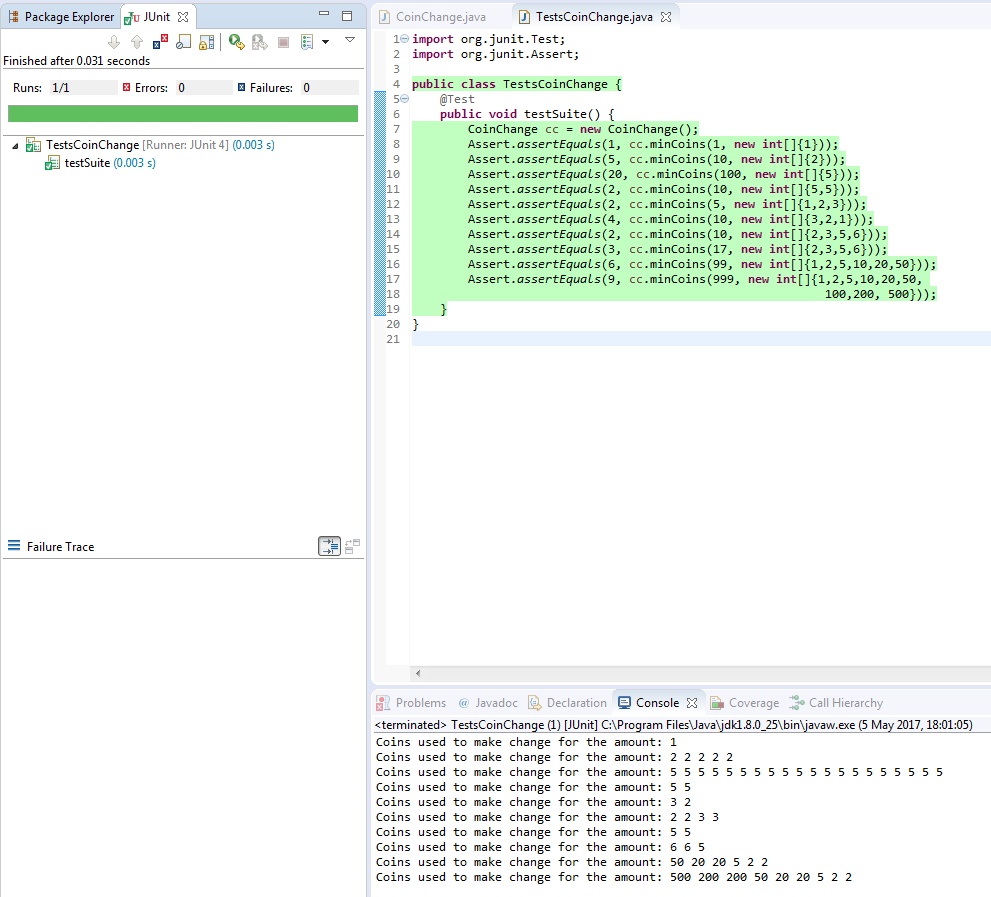
\includegraphics[width=0.8\textwidth]{testing}
	\caption{The test class for minimum coin change problem running Eclemma}
\end{figure}

The final stage of developing the programs was testing. For each program, except for the implementation of the text justification problem, I used EclEmma to perform white-box testing through the Eclipse Java IDE formulated in JUnit. I wrote series of test cases which tested the different sorts of input onto the core methods of each program. Due to the complicated input for the text justification problem, I did testing for that manually myself. The outcome of testing was very positive and by the end of the process I had had concluded that each program was working as intended with no clear errors made in the process. Each test class obtained full coverage over the test cases I created. Through testing I was also able to more clearly evaluate my work, showing the versatility of each problem in terms of input and output.


\section{Technology Choices}
The core technology choice I had to make for this project was with which programming language to write the programs in. I assessed a few different languages to see what advantages they had when it comes to implementation of dynamic programming problems specifically. The biggest advantage any one language that I looked into had was Python, as it allows for memoization to be done automatically, due to functions being first-class objects. This in turn can simplify the implementation of a dynamic programming problem by a fair margin, reducing the amount of code needed. Though a downside of this is that the dynamic programming method is less apparent when looking at the code itself. As I wished for this project to have educational merit and for the code to be as concise as possible, I decided against using Python. The other two programming languages I considered were C++ and Java. Both of these languages have similar functionality in regards to implementation of dynamic programming problems, but I decided against using C++ due to my inexperience with the language. As Java is the language I am most well versed in, I decided it would be the best choice to write my code in. Due to Java being free, open source and platform-independent, it is a very suitable as a choice for the programs I am implementing. There's also the advantage of Java being the most popular programming language in the world by a considerable margin as of April 2017\cite{Java-Pop}, which means it is the most accessible and most likely to be in a potential programmer's skill set.
\smallbreak
I decided against using a GUI library for my code as I felt the nature of the dynamic programming problems I've chosen to implement don't offer too much need for visual representation. In sticking to simple command line input and output, the focus is kept on the algorithms themselves. I did explore the option of designing the programs more with GUI in mind, but felt it would add needless complexity to the usage of the program, having to launch a GUI for a simple format of program which is less time effective than the more basic option of keeping things confined to the command line. Implementing the programs without a GUI component makes them more adaptable and re-usable to potentially be applied within a larger Java program.